\documentclass{article}
\usepackage[utf8x]{inputenc}
\usepackage[colorlinks=true,linkcolor=black,citecolor=blue,pdfusetitle,pagebackref=false]{hyperref}
\usepackage[nonumberlist]{glossaries}
\usepackage{graphicx}
\usepackage{multicol}
\usepackage{caption}
\usepackage{subcaption}
\usepackage{amsmath}
\usepackage{bm}
\usepackage[margin=1.5cm]{geometry}
\usepackage{cite}
\usepackage[usenames,dvipsnames,svgnames,table]{xcolor}
\usepackage{bigints}

\newenvironment{Figure}
  {\par\medskip\noindent\minipage{\linewidth}}
  {\endminipage\par\medskip}

\bibliographystyle{unsrt}
\renewcommand\refname{References}

\newacronym{cdi}
    {CDI}{coherent diffractive imaging}

\newacronym{odt}
    {ODT}{optical dipole trap}

\newacronym{bec}
    {BEC}{Bose-Einstein condensate}

\newacronym{fort}
    {FORT}{far-off-resonance trap}

\newacronym{ta}
    {TA}{tapered amplifier}

\newacronym{caes}
    {CAES}{cold-atom electron source}

\newacronym{xfel}
    {XFEL}{x-ray free electron laser}

\newacronym{mot}
    {MOT}{magneto-optical trap}

\newacronym{ecdl}
    {ECDL}{external cavity diode laser}

\newacronym{aom}
    {AOM}{acousto-optical modulator}

\newacronym{slm}
    {SLM}{spatial light modulator}

\newacronym{mopa}
    {MOPA}{master-oscillator power amplifier}

\newacronym{na}
    {NA}{numerical aperture}

\newacronym{ar}
    {AR}{anti-reflection}

\newacronym{ccd}
    {CCD}{charge-coupled device}

\newacronym{cro}
    {CRO}{cathode ray oscilloscope}

\newacronym{pbs}
    {PBS}{polarising beam splitter}

\newacronym{bs}
    {BS}{beam splitter}

\newacronym{npbs}
    {NPBS}{non-polarising beam splitter}

\newacronym{tec}
    {TEC}{thermo-electric cooler}

\newacronym{cw}
    {CW}{continuous wave}

\newacronym{mcp}
    {MCP}{microchannel plate}

\newacronym{fwhm}
    {FWHM}{full-width half maximum}

\newacronym{pdh}
    {PDH}{Pound-Drever-Hall}
    
\newacronym{ps}
    {PS}{polarisation spectroscopy}
    
\newacronym{obe}
    {OBE}{optical Bloch equation}
    
\newacronym{davll}
    {DAVLL}{dichroic atomic vapour laser lock}

\newacronym{mts}
    {MTS}{modulation transfer spectroscopy}

\newacronym{snr}
    {SNR}{signal-to-noise ratio}

\newacronym{lsd}
    {LSP}{linear spectral density}


\makeglossaries

\begin{document}
\title{Something about Polarisation Spectroscopy}
\author{Joshua Torrance}

\maketitle

\begin{abstract}
By capitalising on the demonstrably high bandwidth of polarisation spectroscopy locking systems it it possible to achieve linewidths of 15 kHz using standard diode lasers.
\end{abstract}

\begin{multicols}{2}

\section{Intro}
Frequency stabilisation is essential to numerous applications including the cooling and trapping of atoms\cite{uetake_high_2008, ye_stable_2010, akamatsu_narrow_2012}, atomic clocks\cite{ludlow_sr_2008}, high resolution spectroscopy\cite{rafac_sub-dekahertz_2000} and metrology\cite{metcalf_laser_1999, ye_quantum_2008, demtroder_laser_2014}.

Current techniques for minimising laser linewidths range from laser stabilisation with saturated absorption, which can achieve linewidths in the region of 150\,kHz\cite{cuneo_optically_1994}, to elaborate experiments involving extremely high finesse cavities that are able to achieve sub-Hertz linewidths with diode lasers using \gls{pdh} locking\cite{ludlow_compact_2007}.

\Gls{ps}\cite{wieman_doppler-free_1976, demtroder_laser_2014} has much in common with the standard laser locking techinique, saturated absorption spectroscopy\cite{maguire_theoretical_2006, haroche_theory_1972, preston_doppler-free_1996} as both techniques provide a frequency reference that can be used to lock lasers to atomic resonaces.

It has been shown that \gls{ps} can be used to reduce the linewidth of a distributed feedback diode from 2\,MHz to 20\,kHz\cite{torii_laser-phase_2012}. Diode laser locked with \gls{ps} have previously reported wavelengths of 65\,kHz\cite{yoshikawa_frequency_2003}. Our high bandwidth feedback to the laser allows diode laser linewidth below 10kHz {\color{red}(or mebbe a lower number if we're lucky)}.

\begin{itemize}
\item Cost is a factor.
\item Broader locking range
\item Better signal to noise
\end{itemize}

\section{Pol Spec Theory}

{\color{red} I like the way that \cite{yoshikawa_frequency_2003} handles the theory. I'd want to more explicitly mention the polarisation by the pump and it's relation to the energy levels and sub-levels.

How do you calculate the refractive index and absorption coefficient?}

\Gls{ps} uses counterpropagating pump and probe beams from the same laser. The pump beam is circularly polarised and the probe is linearly polarised\cite{wieman_doppler-free_1976, demtroder_laser_2014}. The circularly polarised pump induces birefringence in the medium which is then interrogated by the linearly polarised probe beam. The probe beam's polarisation is rotated due to the birefringence.

The polarisation rotation can be monitored using a balanced polarimeter which consists of a \gls{pbs} and two high-bandwidth detectors. Using a balanced polarimeter provides a background-free signal\cite{pearman_polarization_2002} which is ideal for laser locking.

{\color{red} Models of Pol Spec \cite{do_polarization_2008, harris_polarization_2006, pearman_polarization_2002}

Why is it fast?

This has not mentioned atomic transitions yet.}

\section{Setup}

The experimental setup is depicted in figure \ref{polspec_schematic}. Two separate \gls{ecdl} lasers were individually locked with using \gls{ps} and high bandwidth feedback. A heterodyne measurement was taken to determine the lasers' spectral linewidth. A linewidth measurement using a high finesse cavity was also used to confirm the linewidth of the lasers.

High bandwidth feedback is achieved using high bandwidth detectors in the balanced polarimeter (ThorLabs PDA10A-EC with a bandwidth of 100\,MHz), a high bandwidth servo controllers (NewFocus LB1005 with a bandwidth of 18\,MHz) and high bandwidth modulation inputs to the laser diodes (DC to 100\,MHz on the Toptica DL Pro and {\color{red} something else} on the MOGLabs ECDL).

\begin{Figure}
    \centering
    \captionsetup{type=figure}
    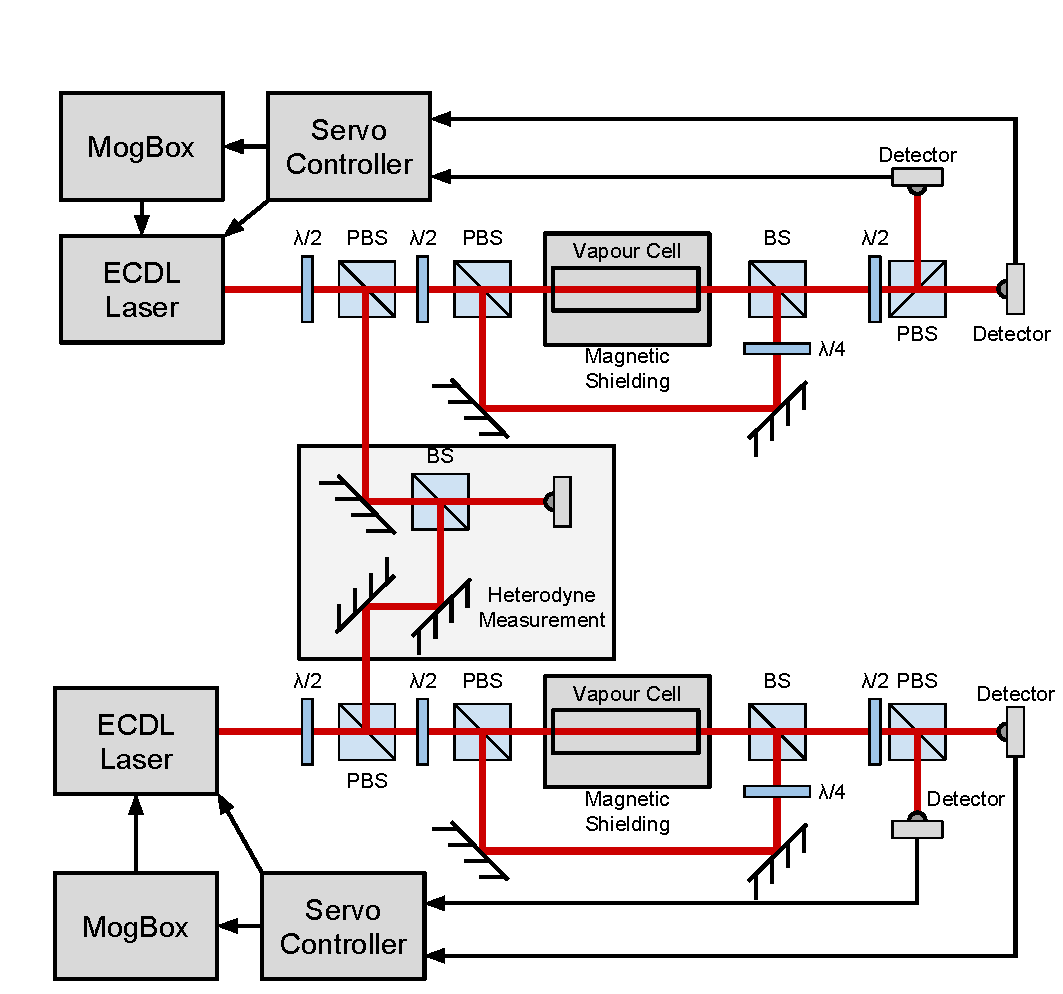
\includegraphics[width=\linewidth]{Figs/FullSimplifiedPolSpecSchematicAttempt.pdf}
    \captionof{figure}{A simplified schematic diagram of the \gls{ps} setup.}
    \label{polspec_schematic}
\end{Figure}

\begin{itemize}
\item describe setup
\item mention fibres or not? ie. how much detail? probably not keep it simple
\end{itemize}

\begin{itemize}
\item bandwidth measurement
\item describe linewidth measurements
    \begin{itemize}
    \item cavity transmission
    \item beatnote
    \end{itemize}
\end{itemize}


\section{Results}
\begin{itemize}
\item bandwidth
\item hetrodyne measurements
\item cavity linewidth measurements
\end{itemize}

\section{Things to consider}
\begin{itemize}
\item Combine setup and results into experiment?
\item Replicate numerical solution in \cite{harris_polarization_2006}?
\end{itemize}

\bibliographystyle{plain}
\bibliography{Library}

\end{multicols}
\end{document}
